\section{Digital Signal Processing}
\label{back:dsp}

The field of \acrfull{dsp} has been researched since the dawn of time. Signals are all around us, and we do have the means to gather and store the data, but how do we process it more efficiently to be able to analyze and interpret the data in a fast and efficient manner?

When working with \acrshort{das} data in particular, we want to filter the data to remove noise, and get cleaner outputs to work with. A common way to remove signals outside of a range are called High-pass filters and Low-pass filters. 

A high-pass filter is a function that only allows frequencies above a certain threshold $T$ to be accepted, while a low-pass filter only accepts frequencies lower than $T$. A band-pass filter on the other hand, only allows frequencies within a certain range to be accepted.

\begin{figure}[h]
\centering
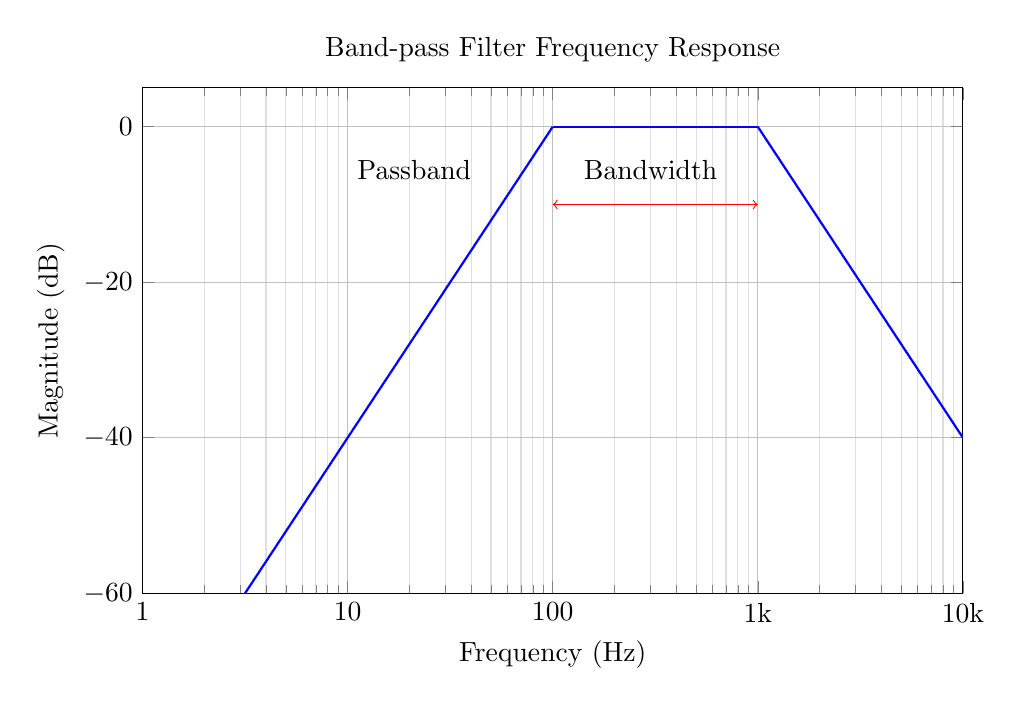
\begin{tikzpicture}
\begin{axis}[
    width=12cm,
    height=8cm,
    xlabel={Frequency (Hz)},
    ylabel={Magnitude (dB)},
    xmode=log,
    xmin=1, xmax=10000,
    ymin=-60, ymax=5,
    xtick={1,10,100,1000,10000},
    xticklabels={1,10,100,1k,10k},
    ytick={-60,-40,-20,0},
    grid=both,
    minor grid style={gray!25},
    major grid style={gray!50},
    title={Band-pass Filter Frequency Response},
]

% Low-frequency rolloff
\addplot[domain=1:100,samples=100,blue,thick] {-40*log10(100/x)};

% Passband
\addplot[domain=100:1000,samples=100,blue,thick] {0};

% High-frequency rolloff
\addplot[domain=1000:10000,samples=100,blue,thick] {-40*log10(x/1000)};

% Annotations
\node[anchor=north west] at (axis cs:10,-3) {Passband};
\draw[<->,red] (axis cs:100,-10) -- (axis cs:1000,-10);
\node[anchor=south] at (axis cs:300,-8) {Bandwidth};

\end{axis}
\end{tikzpicture}
\caption{Ideal Bandpass Filter Response}
\end{figure}


\subsection{Tukey Window}
\label{dsp:tukey}

Window functions are function often used in \acrshort{dsp} to avoid artifacts. This is done by setting values oytside a pre-defined interval to zero and apply a taper from the pass-band to the first zero-value. The Tukey window, also known as the \textit{cosine-tapered window} is one of the more popular window methods, and its mathematical function is described as such: 

\[
    w(x)= 
\begin{cases}
    \frac{1 + \cos{2 \pi \alpha (x + \frac{1-\alpha}{2})}}{2}, & \text{if } x \leq \frac{1-\alpha}{2}\\
    1,              & \text{if } \frac{\alpha}{2} < x \leq \frac{\alpha}{2}\\
    \frac{1 + \cos{2 \pi \alpha (x - \frac{1-\alpha}{2})}}{2}, & \text{if } x > \frac{1-\alpha}{2}
\end{cases}
\]

This window becomes a rectangle when $\alpha = 0$.


\subsection{Resampling}

Also known as sampling-frequency conversion, resampling is the act of modifying the sampling rate of a discrete signal to obtain a new discrete representation of this data. For signal data, lots of samples are usually recorded, but the amount needed to perform calculations or observe patterns does not require this much data. Thus, one can downsample the data to decrease memory usage for storage, as well as time for processing this data. \\

\subsubsection{Parallel Matrix Resampling}

Matrices can be resampled by resampling each vector either row-wise or column-wise. Consequentially, the resulting outputs can be concatenated into a new matrix. These types of matrix operations can be classified as trivial parallelizable, either by using multiple threads or processes. In either case, $n$ workers are created, where each of them get an almost equal amount of vectors to resample, and a \texttt{gather} procedure is then performed to create the output matrix. This is further illustrated in figure \ref{fig:parres}.

\begin{figure}[h]
    \centering
    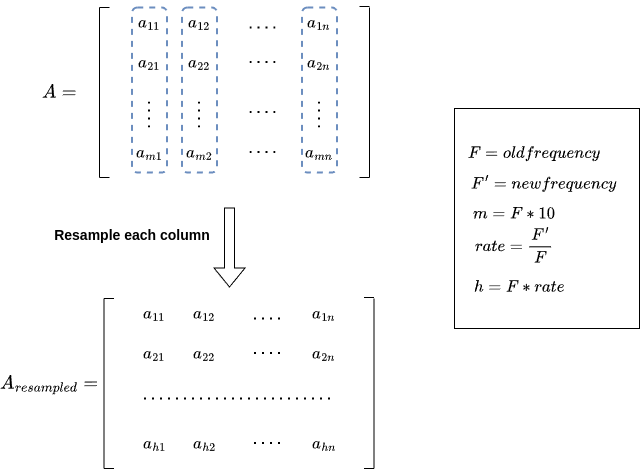
\includegraphics[width=0.8\linewidth]{figures/parallel_resample.png}
    \caption{Showcase of how columnwise resampling of a matrix can be parallellized}
    \label{fig:parres}
\end{figure}
